\documentclass[tikz,border=6pt]{standalone}
\usepackage{amsmath}
\usetikzlibrary{calc}
\definecolor{cA}{RGB}{31,94,165}\definecolor{cB}{RGB}{214,96,33}\definecolor{cC}{RGB}{46,139,87}
\tikzset{
  va/.style={circle,inner sep=0pt,minimum size=9pt,ball color=cA!40,draw=cA!80!black,line width=0.25pt},
  vb/.style={circle,inner sep=0pt,minimum size=9pt,ball color=cB!40,draw=cB!80!black,line width=0.25pt},
  vc/.style={circle,inner sep=0pt,minimum size=9pt,ball color=cC!40,draw=cC!80!black,line width=0.25pt},
  vh/.style={circle,inner sep=0pt,minimum size=12pt,ball color=yellow!70!orange,draw=black!70,line width=0.4pt},
  faint/.style={line width=0.25pt,black!13},
  hot/.style={line width=1.0pt,black!75},
  mt/.style={line width=1.0pt,black!75,densely dashed},
  vl/.style={font=\scriptsize,inner sep=0.5pt}}
\begin{document}
% H_21 on a tilted ring: the cyclic order a_0..a_6, c_0..c_6, b_0..b_6 (vertex v of H_21 is
% a_i = 3i, b_i = 3i+1 or c_i = 3i+2). Vertices at cyclic distance 8..13 are adjacent, at distance
% 1..6 not; at distance 7 only the pairs a_i c_i are adjacent.
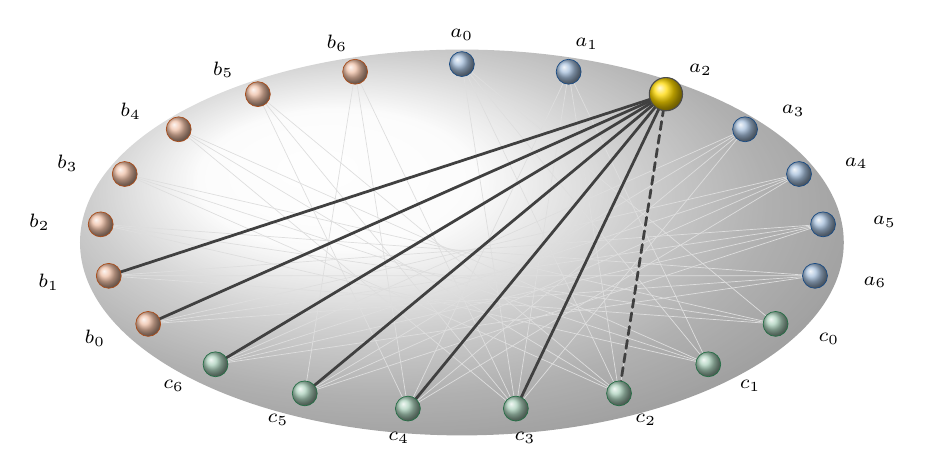
\begin{tikzpicture}[x={(4.6cm,0cm)},y={(0cm,2.2cm)},z={(0cm,0.55cm)},line cap=round]
\shade[ball color=black!3,opacity=0.6] (0,0,-0.12) ellipse [x radius=4.85cm,y radius=2.45cm];
\foreach \p in {0,...,20}{\coordinate (P\p) at ({cos(90-360*\p/21)},{sin(90-360*\p/21)},0);}
% every edge, faint: cyclic distance 8..10 (the largest possible is 10)
\foreach \p in {0,...,20}{\foreach \d in {8,9,10}{
  \pgfmathtruncatemacro{\q}{mod(\p+\d,21)}
  \ifnum\p<\q \draw[faint] (P\p) -- (P\q);\fi}}
% the matching a_i c_i (cyclic distance 7)
\foreach \i in {0,...,6}{\pgfmathtruncatemacro{\q}{\i+7}\draw[faint] (P\i) -- (P\q);}
% the neighbourhood of a_2 (position 2): c_2 (matched) and c_3..c_6, b_0, b_1
\draw[mt] (P2) -- (P9);
\foreach \q in {10,11,12,13,14,15}{\draw[hot] (P2) -- (P\q);}
\foreach \i in {0,...,6}{\node[va] at (P\i) {};}
\foreach \i in {7,...,13}{\node[vc] at (P\i) {};}
\foreach \i in {14,...,20}{\node[vb] at (P\i) {};}
\node[vh] at (P2) {};
\foreach \i in {0,...,6}{
  \pgfmathtruncatemacro{\c}{\i+7}\pgfmathtruncatemacro{\b}{\i+14}
  \node[vl] at ($(P\i)!-0.17!(0,0,0)$) {$a_{\i}$};
  \node[vl] at ($(P\c)!-0.17!(0,0,0)$) {$c_{\i}$};
  \node[vl] at ($(P\b)!-0.17!(0,0,0)$) {$b_{\i}$};}
\end{tikzpicture}
\end{document}
